\documentclass{standalone}
\usepackage{../../../../preamble_tikz}

\begin{document}

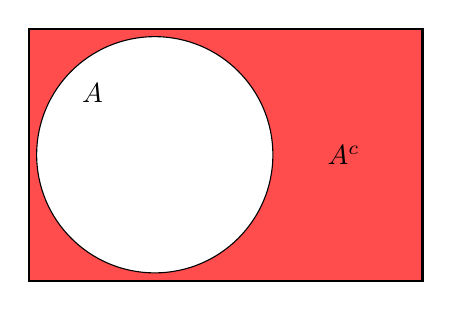
\begin{tikzpicture}
  \draw[fill=red!70,thick] (-1.6,-1.6) rectangle (3.4,1.6);
  % Set A
  \node[circle,minimum size = 3cm,label={[label distance=-0.75cm]135:$A$},fill=white] (A) at (0,0) {}; %"minimum size" is the diameter. "label={135:$A$}" positions texts $A$ at 135 degrees of the circle. 

  % Draw circle outline
  \draw (0,0) circle(1.5cm);

  % Set intersection label
  \node at (2.4,0) {$A^c$};

\end{tikzpicture}
\end{document}